\chapter{Discrete Event Simulator}
\label{cha:des}

Experiments on \ac{BGP} are not applicable on the Internet, for this
reason different studies show their results using a simulate environment
\cite{griffin2001experimental} \fxfatal{Insert other citations}.
The majority of the studies uses small graphs and each node 
of the graph simulate the behaviour of a \ac{BGP} speaker.
Each node represent also a single \ac{AS} and the \ac{BGP} speaker is it's own
exterior router, for simplicity, reduced to one speaker that handles all the
connections. 
 
For this reason, I decided to use and expand a \ac{DES} that permits to have
different grades of freedom, respecting on the other side all the properties
required for a reliable simulator environment.
I decided to use the \textit{Simpy}\footnote{\href{https://simpy.readthedocs.io/en/latest/index.html}{Simpy website}}
package to make the environment evolve. I decided for this package for the
extensive documentation and because it has been already used for different
studies, demonstrating its adaptability \cite{matloff2008introduction,dagkakis2013manpy}.

I developed the \ac{DES} as a highly modular environment.
\begin{figure}[h]                                                               
    \begin{center}                                                              
        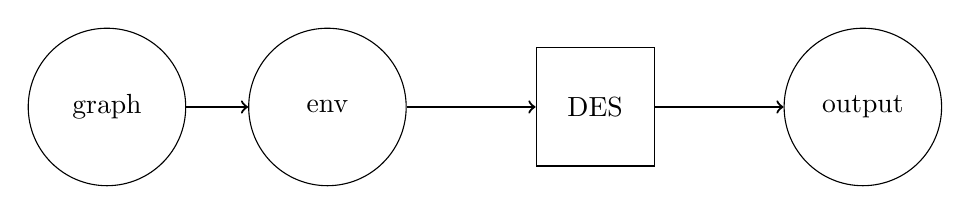
\begin{tikzpicture}[scale=0.2, every node/.style={draw=black,circle,inner sep=0pt}]
    \node [minimum size=2cm] (graph) at (0,0) {graph}; 
    \node [minimum size=2cm] (env) at (14,0) {env};                                    
    \node [rectangle, draw, minimum width=1.5cm,minimum height=1.5cm] (des) at (31,0) {DES};
    \node [minimum size=2cm] (output) at (48,0) {output};                                    
    \draw [thick, ->] (graph) to (env);                                  
    \draw [thick, ->] (env) -- (des);                                 
    \draw [thick, ->] (des) -- (output);                                 
\end{tikzpicture}                                                       

    \end{center}                                                                
    \caption{Discrete event simulator structure}                                
    \label{fig:des_structure}                                                   
\end{figure}

In \Cref{fig:des_structure} is possible to see the basic idea of the simulator.
The first component needed is a graph, represented by a \textit{graphml} file, 
this file is the descriptor of the network. 
it defines also all topological information and all the properties of every single node.
In Code \ref{lst:graph_example} is possible to see an example of a \textit{graphml} file,
it describes that node \num{0} contains a single destination and that the edge
between nodes \num{2} and \num{5} is controlled by the policy |2, 2, 2| that defines
a servicer-provider policy.
Policies are encoded using the convention described in \cite{daggitt2018rate}.

\lstcaptionname{Code}
\begin{lstlisting}[language=graphml, caption=Graph example, label=lst:graph_example]
 <node id="0">
      <data key="d0">10.0.0.0/24</data>
 </node>
 <edge source="2" target="5">                                                  
     <data key="d2">2, 2, 2</data>                                             
 </edge> 
\end{lstlisting}

The graph is then embedded in the environment file, this file is in \textit{JSON}
format and it describes how the environment is characterized, it gives the 
initial values for the \ac{RNG} so that each experiment is replicable and
other properties, like where the output should be saved, and, most importantly
how the experiment should be conducted.
There is two possible evolution of the environment:
\begin{itemize}
    \item \textbf{\textit{Continuous evolution}}: In this category all the nodes
    that contains at least a destination will continuously share and retrieve
    the destination accordingly with the distributions defined in the environment;
    \item \textbf{\textit{Signaling evolution}}: Is possible to define a precise
    signal that should be executed by the nodes that contain a destination, for 
    example, the signal \q{AWA} defines that there will be an announce followed by 
    a withdraw and another announce.
\end{itemize}

The \ac{DES} take as input this \textit{JSON} file where all the information
are described, it creates an object for each node in the graph file, with
each own characteristics.
After the initialization, all the nodes that contain a destination will schedule
the first advertisement of it to their neighbour.
The simulation run will terminate only if there are no more events scheduled or
if the maximum simulation time is reached.

The \ac{DES} will then produce a \textit{CSV} output, with all the events that 
can be analyzed to see the evolution of a specific node or to evaluate the
whole network.
 
\section{DES Environments}
\label{sec:des_environment}

Thanks to the environment codification in a \textit{JSON} file is possible to
define experiments with a high grade of freedom. 
Is possible to define multiple delays as probability functions vectors that
will provide multiple runs possibility. For example, if we have \num{5} different
possible seeds and \num{3} different delays, the total number of runs combinations
is \num{15}, as shown in Code \ref{lst:environment_example}.
is possible to run one of the possible combinations of parameters through the identifier
of the single run.

\lstcaptionname{Code}
\begin{lstlisting}[language=json, caption=Environment example, label=lst:environment_example]
"simulation" : {                                                              
    // seed(s) to initialize RNG                                      
    "seed" : [0, 1, 2, 3, 4], 
    ....
    // Multiple withdraw distributions
    "withdraw_dist": [{"distribution": "unif", "min": 5, "max": 10, "int": 0.1},
                      {"distribution": "unif", "min": 8, "max": 10, "int": 0.1},
                      {"distribution": "unif", "min": 2, "max": 3, "int": 0.1}],       
    ....
}
\end{lstlisting}

In the environment is possible to define also the processing time, this time is used
inside each \ac{BGP} node to emulate the processing of information or the evaluation
of a packet.
Though the \textit{delay} parameter is possible to define the default delay on the edges,
is important to remember that the links are FIFO so there is no reordering
of messages in the same link, there is also no messages lost.
That because it was out of the scope of this thesis to study the evolution
of the protocol with packet loss, but it could be future work.

\subsection{Clique environment}
\label{subsec:clique_env}

One of the special environment that I used in my experiments uses clique 
graphs of different dimensions, an example of the clique graph is given in
\Cref{fig:clique_topology}.

The only node that shares a destination is the node \q{\textit{d}}, the node
\num{0} will then spread the knowledge to the whole network, and the node 
\q{\textit{x}} will act as a black hole for all the possible paths
that the node \num{5} will share.

This topology is used to enforce the \textit{Path exploration} problem, it also
gives the possibility to study how \ac{BGP} parameters can influence the messages
distribution in stressful cases like the clique one.
I'm going also to study how the variation of those parameters from the standard
ones can impact the performances in this environment of high load.

\subsection{Fabrikant environment}
\label{subsec:fabrikant_env}

Another interesting chase to test the path exploration problem is the one
presented in \cite{fabrikant2011there}.
In that study, Fabrikant et al. presents how particular \ac{MRAI} setting could 
make the network converge with exponential behaviour because of the 
continuous decision change in terms of best paths from the nodes. 
I used the basic example of their study to investigate how the choice of \ac{MRAI}
is fundamental for the network convergence.
An example of the network used is presented in \Cref{fig:fabrikant_topology}.

The path exploration problem is caused by the delay on the \num{0}-\num{2}
edge. The node \num{2} will receive the destination through node \num{1}, after a small amount
of time the network will converge to the best path (without using the backup links).
But, after a while, node \num{2} will receive the network also through node \num{0}
and it will prefer this new path, provoking then the reconfiguration of all
the other nodes that will use the backup links for a while, announcing their 
new paths.
A wrong configuration of \ac{MRAI} can provoke the entire exploration of the 
possibility set.

This environment is also used to show how a \ac{BGP} \ac{FSM} would explode
in terms of possible states and edges producing an enormous ammount of possible
output signals from the same input.

\subsection{Internet-like environment}
\label{subsec:internet_like_env}

The last noteworthy environment is the one whose purpose is to simulate the Internet
behaviour.
This has been possible thanks to the study by Elmokashfi et al. \cite{elmokashfi2010scalability}
and the internet like graph generator present in Networkx \footnote{\href{https://networkx.org/documentation/stable/reference/generated/networkx.generators.internet_as_graphs.random_internet_as_graph.html\#networkx.generators.internet_as_graphs.random_internet_as_graph}{Networkx internet as graph generator}}
(a Python library famous for graph and network studies).
An example with a small set of nodes is presented in \Cref{fig:internet_like_topology}.

The different nodes are coloured accordingly with the node type represented.
The tier one nodes that generate the central clique are coloured in red and
is possible to notice in \Cref{fig:internet_topology_hierarchical} that they are
in the highest levels of the networks.
This environment has been used to study the behaviour of the network with 
topologies resembling the real internet.

In the next studies, I generally refer to this kind of topology with the 
terms \q{Internet-like}, and the dimension is never less than \num{1000} nodes,
otherwise is not possible to ensure all the Internet topological properties.

The goal of the experiments that use that kind of topologies is to study
the general network performances in terms of average convergence time and 
the number of messages transmitted.
This would help to see and study behaviours that are more typical in the actual
Internet.
